
\section{datAcron Architecture}		
\frame
{		
	\frametitle{datAcron Architecture}
	\framesubtitle{}
	
	\begin{center}
		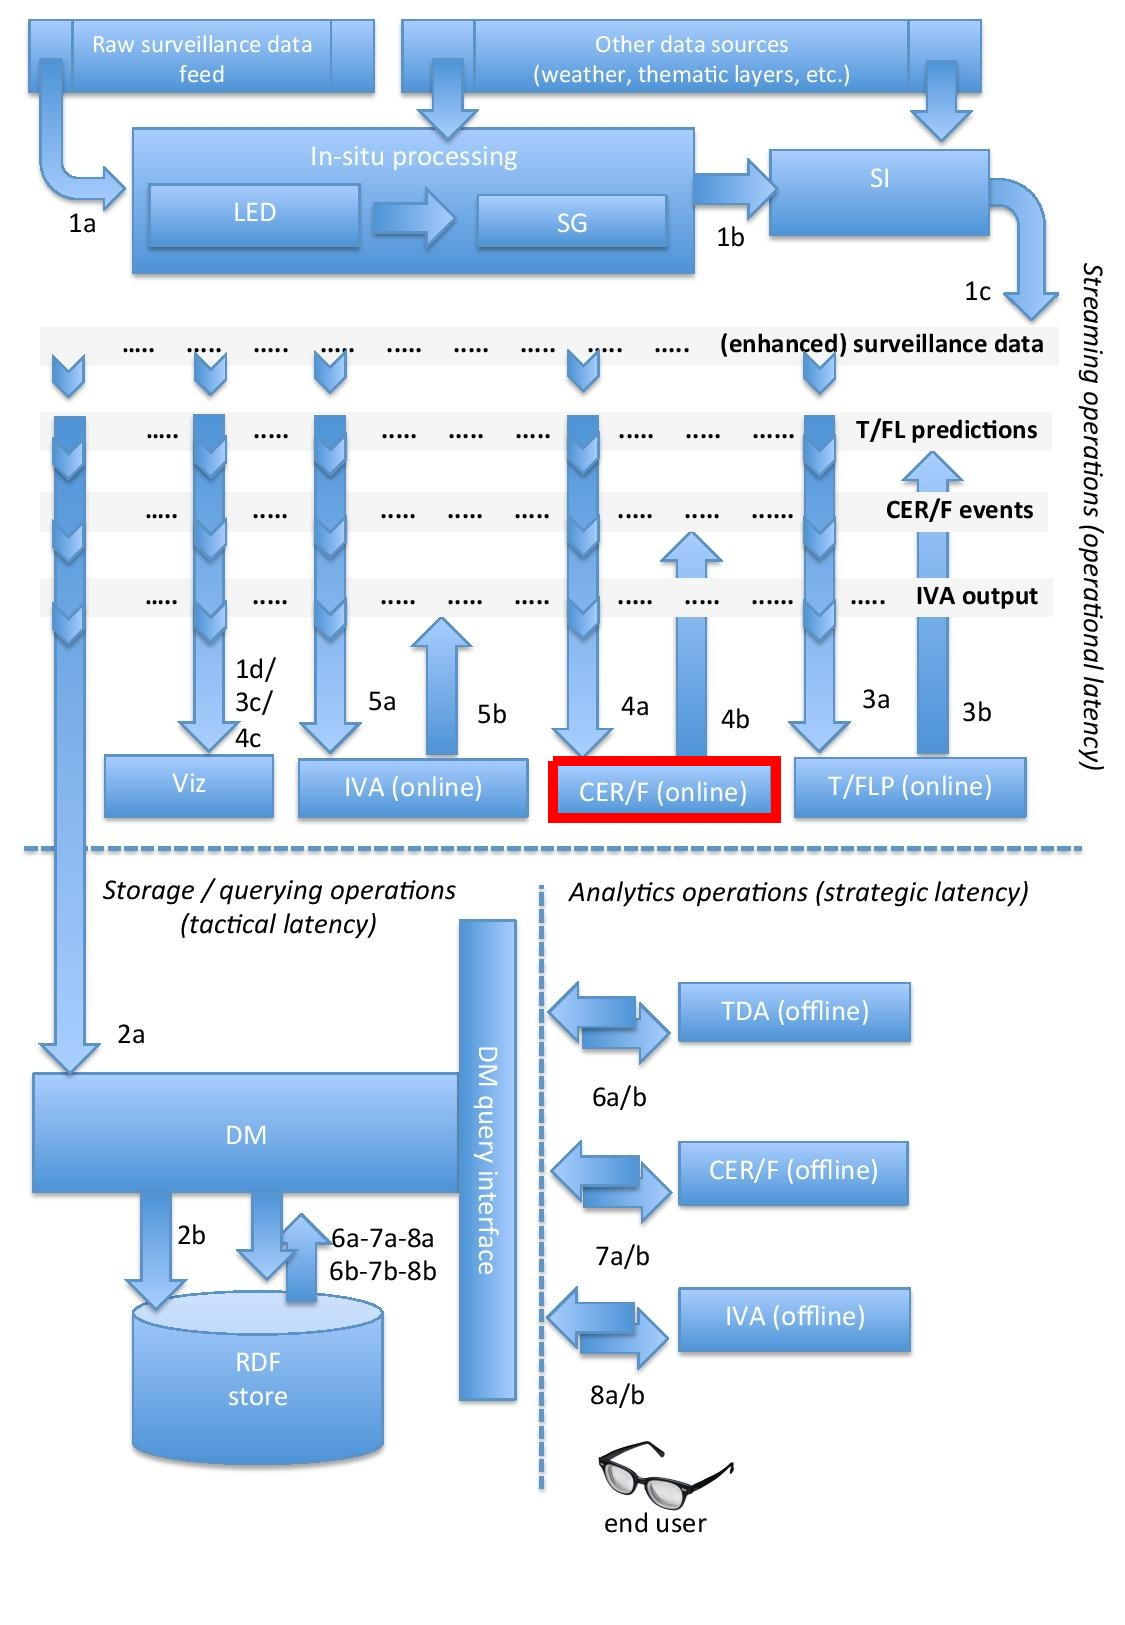
\includegraphics[width=.85\textwidth,height=.75\linewidth]{figures/arch2.jpg}\\
		.
	\end{center}
	
}
\section{Proposed Approach}
\frame
{
	\frametitle{Problem Setting}
	
	\begin{itemize}[]
		\item<1->Given a set of $k$ real-time streams of events $S = \{ s_1,s_2, ..., s_k\}$.
		
		\item<1 -> Each stream $s_i=\langle e_1,e_3...,e_t,...\rangle$  is an evolving time-ordered sequence of events.
		
		\item<1 -> Each event is defined as a tuple of attributes $e_t = (type,\tau,id,a_1,a_2.....,a_n)$ where $type\ \in  \Sigma$ (i.e., event types). 
		\item<1-> A user-defined pattern (i.e., complex event of interest) $P$ expressed as sequence of event types.
		
		%  \item<1->Goal:  provides online prediction about when the event pattern $P$ is expected to be completed each single stream $s_i$ 
		
		\item<1->Goal: the main objective is to predict the pattern $P$ completion with certain probability in the future over each stream $s_i$ given the current time event $e_t$. 
	\end{itemize}
}

\begin{frame}[fragile]
	
	\frametitle{Maritime Surveillance}
	\framesubtitle{}
	\begin{itemize}
		%		\item<only@1> Process  emitted from moving vessels or derived critical points of vessel trajectories as input event streams.
		\item<only@1> Event tuple (i.e., critical points) derived from raw Automatic Identification System (AIS) messages of moving vessels e.g., 
		\begin{minted}{json}
		{
		"timestamp":1443651492000,
		"id":"228133000",
		"annotation":"change_in_heading",
		"latitude":48.117775,
		"longitude":-4.4205885,
		"distance":323.406,
		"heading":264.27
		"speed":18.48,
		}
		\end{minted}
		
		\item<only@1> Example patterns such as 
		$P_1=\mathit{change\_heading} \cdot \mathit{gap\_start} \cdot \mathit{gap\_end} \cdot 
		\mathit{change\_heading}$ or $P_2=\mathit{Sailing}$
	\end{itemize}
\end{frame}


\frame
{
	\frametitle{A Distributed Online Learning Approach for Large-scale Pattern Prediction \footnote{Source Code: https://goo.gl/xwX1Mk}}
	%\framesubtitle{Maritime Surveillance}
	\framesubtitle{Distributed Architecture (Qadah, E., Mock, M., Alevizos, E. \& Fuchs, G. (n.d.))}
	\begin{center}
		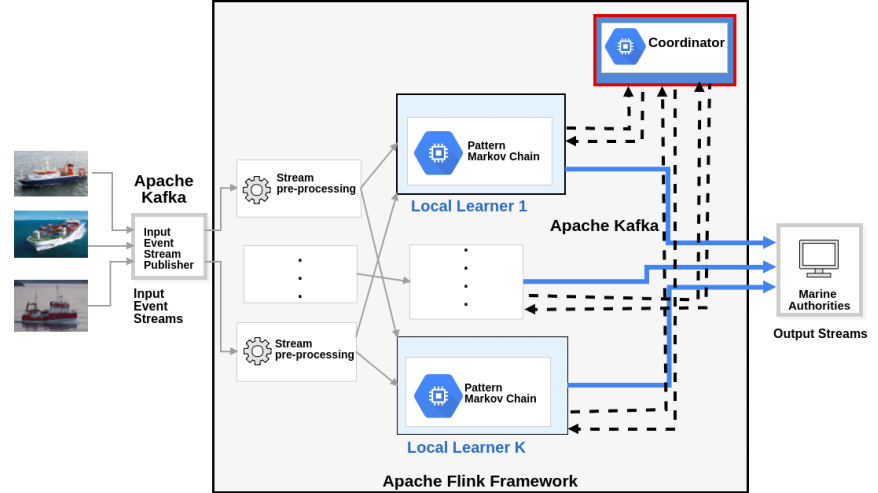
\includegraphics[width=1.05\textwidth,left,height=.58\linewidth]{figures/distributed_architecture_2.png}
.
	\end{center}
}

\subsection{\\ Event Forecasting with Pattern Markov
	Chains\\}
\frame
{
	\frametitle{ Event Forecasting with Pattern Markov
		Chains}
	\framesubtitle{\citep{alevizos2017event}}
	\begin{itemize}[]
		\item<1-> The system consumes a single input stream $s_i$ of events.
		\item<1-> The event stream $s_i$ is assumed to be generated by  $m$-order Markov source.
		\item<1-> The complex event (i.e., pattern) $P$ is defined in the form of regular expressions over a finite set of event types $\Sigma$.
		
		\item<1-> A probabilistic model provides online forecasting reports when the event pattern $P$ is expected to be completed in future. 
		
	\end{itemize}
}


\frame
{
	\frametitle{Event Forecasting with Pattern Markov
		Chains}
	\framesubtitle{How does it work?}
	\begin{itemize}
		\item<only@1> The  deterministic finite automa ($DFA$) is used to construct a Markov chain, which is called a Pattern Markov Chain (PMC).
		
		
		\item<only@1> The states of $DFA$ is directly mapped to states of  transition probability matrix $\boldsymbol{M}$  $\lvert Q \rvert \times \lvert Q \rvert$ of the $PMC$.
		
		\item<only@1> 
		\begin{equation*}
		\label{eq:matrix_example}
		\boldsymbol{M} = 
		\begin{Bmatrix} 
		0 \\ 1 \\ 2 \\ 3 \\4
		\end{Bmatrix}
		\begin{pmatrix} 
		p_{0,0}	    &. 		&. 		& . &  	p_{0,4} \\
		. 		    & .		& .	& .	& . \\
		.		    & .		& .		& .	& . \\
		.			& .		& .		& .	& .\\
		0			& .			& .		& .	&p_{4,4}
		\end{pmatrix}
		\end{equation*}
		
		\item<only@1> The maximum-likelihood estimator is used to compute the transition probabilities (i.e., learning) $p_{i,j}$ of the matrix $\boldsymbol{M}$ 
		\begin{equation}
		\label{eq:pi_estim}
		\hat{p}_{i,j}=\frac{n_{i,j}}{\sum_{k \in Q} n_{i,k}}=\frac{n_{i,j}}{n_{i}}
		\end{equation}. 	
		
	\end{itemize}
}

\subsection{Communication-Efficient Distributed Online Prediction by Dynamic Model Synchronization}
\frame
{
	\frametitle{ Communication-Efficient Distributed Online Prediction by Dynamic Model Synchronization  }
	\framesubtitle{\citep{kamp2014communication}}
	\begin{itemize}[]
		\item<1-> A protocol for distributed online prediction over multiple input data streams in a communication efficient manner.
		\item<1-> It allows to combine local models into a global model
	using a $synchronization$ $ operation$.
		\item<1-> The distributed learners exchange their local model with a central coordinator node periodically after observing a fixed number of data points (i.e., mini-batches) \citep{dekel2012optimal}.
		
		\item<1-> A dynamic synchronization scheme based on monitoring the local models variance from a global reference model ($\|f_i - r\|^2 \leq \bigtriangleup$).
		
		
%		dynamic synchronization scheme within which the learners communicate only if their local models diverge from a global reference point
	\end{itemize}
}


\frame
{
	\frametitle{ Communication-Efficient Distributed Online Prediction by Dynamic Model Synchronization}
	\framesubtitle{}
	\begin{center}
		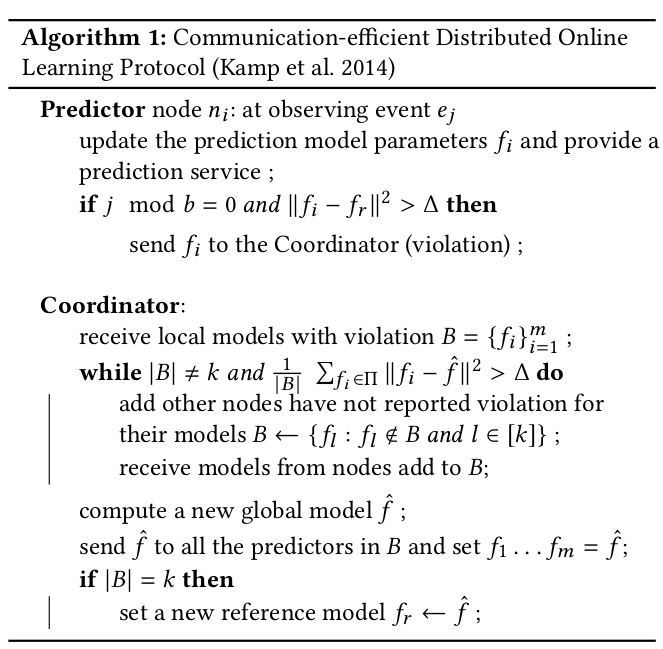
\includegraphics[width=\textwidth,left,height=.8\textheight]{figures/dol.png}\\
		.
	\end{center}
}

\frame
{
	\frametitle{A Distributed Online Learning Approach for Large-scale Pattern Prediction}
		\framesubtitle{Synchronization Operation}
	\begin{itemize}[]

	\item<1->\ We propose a \textit{synchronization operation} for the parameters of the models ($f_i=\boldsymbol{\Pi}_i :i \in[k]$) of the $k$ distributed PMC predictors. The operation is based on distributing the maximum-likelihood estimation for the transition probabilities of the underlying  models described by: 
	\begin{equation*}
	\label{eq:dis_pi_estim}
	\hat{\pi}_{i,j}=\frac{\sum_{k \in K} n_{k,i,j}}{\sum_{k \in K} \sum_{l \in L} n_{k,i,l}}
	\end{equation*}
	
\item<2-> We measure the divergence of local models from the reference model  $\|f_k - f_r\|^2$ by calculating the sum of square difference between the transition probabilities  $\boldsymbol{\Pi}_i$ and  $\boldsymbol{\Pi}_r$:
	\begin{equation*}
	\label{eq:dis_pi_varinace}
	\|f_k - f_r\|^2=\sum_{i,j} (\hat{\pi}_k{i,j} -\hat{\pi}_r{i,j})^2
	\end{equation*}

	
\end{itemize}
}